% Automata Course. Week 2, Question 4: Convert Regular Expression to epsilon-NFA
\documentclass[preview,11pt]{standalone}
\usepackage[svgnames]{xcolor}
\usepackage{tikz}
\usetikzlibrary{automata,shapes,backgrounds,arrows,positioning,fit,calc}
\begin{document}
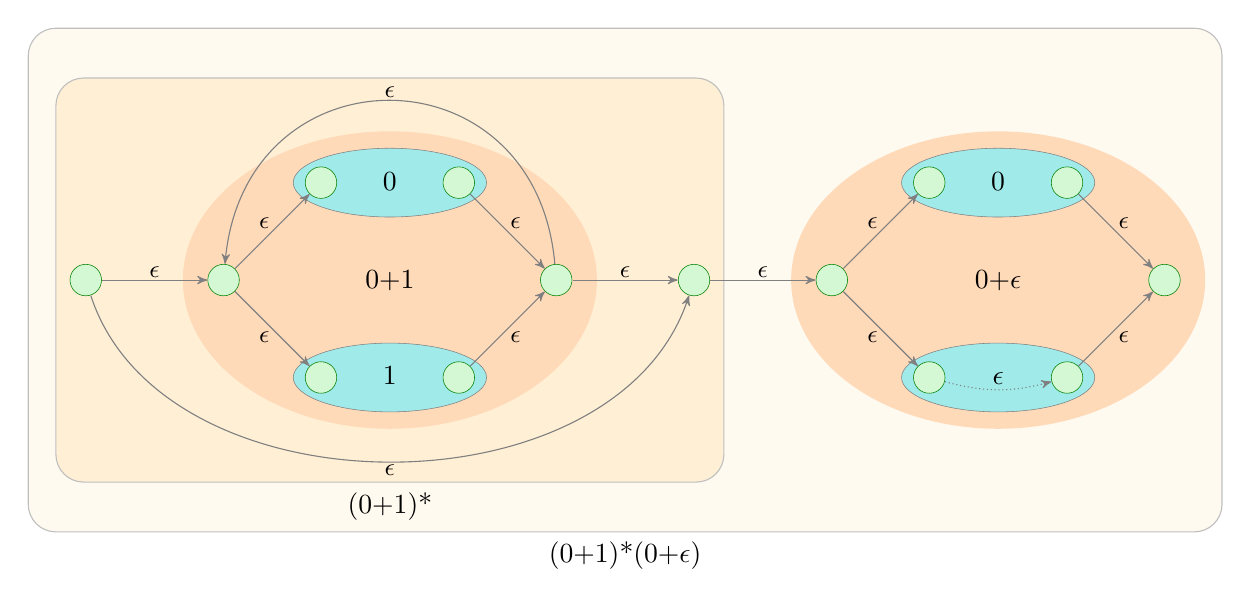
\begin{tikzpicture}[
  on grid,auto,
  ->, >=stealth',shorten <=0.10pt,shorten >=0.10pt,
  node distance=1.75cm,thin,
  every state/.style={very thin,draw=Green,fill=LightGreen!40,inner sep=0,
    minimum size=4mm},
  every edge/.style={draw=Gray,font=\sffamily\small,inner sep=0.85pt},
  automaton1/.style={ellipse,very thin,draw=Gray,fill=PaleTurquoise!120,
    inner xsep=-6pt,inner ysep=3pt,text height=8.5pt},
  automaton2/.style={ellipse,very thin,fill=PeachPuff,
    inner xsep=-13pt,inner ysep=-3pt,text height=44pt},
  automaton3/.style={rounded corners=10pt,draw=Gray!50,fill=PapayaWhip,
    inner xsep=5pt,inner ysep=32pt},
  automaton4/.style={rounded corners=10pt,draw=Gray!50,fill=FloralWhite,
    inner xsep=15pt,inner ysep=50pt}
  ]

  \node[state] (q01)                      {};
  \node[state] (q02) [right=of q01]       {};
  \node[state] (q03) [above right=of q02] {};
  \node[state] (q04) [below right=of q02] {};
  \node[state] (q05) [right=of q03]       {};
  \node[state] (q06) [right=of q04]       {};
  \node[state] (q07) [below right=of q05] {};
  \node[state] (q08) [right=of q07]       {};
  \node[state] (q09) [right=of q08]       {};
  \node[state] (q10) [above right=of q09] {};
  \node[state] (q11) [below right=of q09] {};
  \node[state] (q12) [right=of q10]       {};
  \node[state] (q13) [right=of q11]       {};
  \node[state] (q14) [below right=of q12] {};

  \begin{scope}[on background layer]
    \node[automaton4,fit=(q01)(q02)(q03)(q04)(q05)(q06)(q07)(q08)(q09)(q10)
      (q11)(q12)(q13)(q14),label=below:(0+1)*(0+$\epsilon$)] {};

    \node[automaton3,fit=(q01)(q02)(q03)(q04)(q05)(q06)(q07)(q08),
      label=below:(0+1)*] {};

    \node[fit=(q02)(q03)(q04)(q05)(q06)(q07),automaton2] {0+1};
    \node[fit=(q09)(q10)(q11)(q12)(q13)(q14),automaton2] {0+$\epsilon$};

    \node[fit=(q03)(q05),automaton1] {0};
    \node[fit=(q04)(q06),automaton1] {1};
    \node[fit=(q10)(q12),automaton1] {0};
    \node[fit=(q11)(q13),automaton1] {$\epsilon$};
  \end{scope}
  
  \path[->,Black] 
    (q01) edge []                             node        {$\epsilon$} (q02)
    (q01) edge [bend right=72]                node [swap] {$\epsilon$} (q08)
    (q02) edge []                             node        {$\epsilon$} (q03)
    (q02) edge []                             node [swap] {$\epsilon$} (q04)
    (q05) edge []                             node        {$\epsilon$} (q07)
    (q06) edge []                             node [swap] {$\epsilon$} (q07)
    (q07) edge []                             node        {$\epsilon$} (q08)
    (q07) edge [bend right=85,looseness=1.70] node [swap] {$\epsilon$} (q02)
    (q08) edge []                             node        {$\epsilon$} (q09)
    (q09) edge []                             node        {$\epsilon$} (q10)
    (q09) edge []                             node [swap] {$\epsilon$} (q11)
    (q11) edge [densely dotted,bend right=15] node [swap] {}           (q13)
    (q12) edge []                             node        {$\epsilon$} (q14)
    (q13) edge []                             node [swap] {$\epsilon$} (q14)
    ;
\end{tikzpicture}
\end{document}
